\documentclass[11pt,preprint, authoryear]{elsarticle}

\usepackage{lmodern}
%%%% My spacing
\usepackage{setspace}
\setstretch{1.2}
\DeclareMathSizes{12}{14}{10}{10}

% Wrap around which gives all figures included the [H] command, or places it "here". This can be tedious to code in Rmarkdown.
\usepackage{float}
\let\origfigure\figure
\let\endorigfigure\endfigure
\renewenvironment{figure}[1][2] {
    \expandafter\origfigure\expandafter[H]
} {
    \endorigfigure
}

\let\origtable\table
\let\endorigtable\endtable
\renewenvironment{table}[1][2] {
    \expandafter\origtable\expandafter[H]
} {
    \endorigtable
}


\usepackage{ifxetex,ifluatex}
\usepackage{fixltx2e} % provides \textsubscript
\ifnum 0\ifxetex 1\fi\ifluatex 1\fi=0 % if pdftex
  \usepackage[T1]{fontenc}
  \usepackage[utf8]{inputenc}
\else % if luatex or xelatex
  \ifxetex
    \usepackage{mathspec}
    \usepackage{xltxtra,xunicode}
  \else
    \usepackage{fontspec}
  \fi
  \defaultfontfeatures{Mapping=tex-text,Scale=MatchLowercase}
  \newcommand{\euro}{€}
\fi

\usepackage{amssymb, amsmath, amsthm, amsfonts}

\def\bibsection{\section*{References}} %%% Make "References" appear before bibliography


\usepackage[round]{natbib}

\usepackage{longtable}
\usepackage[margin=2.3cm,bottom=2cm,top=2.5cm, includefoot]{geometry}
\usepackage{fancyhdr}
\usepackage[bottom, hang, flushmargin]{footmisc}
\usepackage{graphicx}
\numberwithin{equation}{section}
\numberwithin{figure}{section}
\numberwithin{table}{section}
\setlength{\parindent}{0cm}
\setlength{\parskip}{1.3ex plus 0.5ex minus 0.3ex}
\usepackage{textcomp}
\renewcommand{\headrulewidth}{0.2pt}
\renewcommand{\footrulewidth}{0.3pt}

\usepackage{array}
\newcolumntype{x}[1]{>{\centering\arraybackslash\hspace{0pt}}p{#1}}

%%%%  Remove the "preprint submitted to" part. Don't worry about this either, it just looks better without it:
\makeatletter
\def\ps@pprintTitle{%
  \let\@oddhead\@empty
  \let\@evenhead\@empty
  \let\@oddfoot\@empty
  \let\@evenfoot\@oddfoot
}
\makeatother

 \def\tightlist{} % This allows for subbullets!

\usepackage{hyperref}
\hypersetup{breaklinks=true,
            bookmarks=true,
            colorlinks=true,
            citecolor=blue,
            urlcolor=blue,
            linkcolor=blue,
            pdfborder={0 0 0}}


% The following packages allow huxtable to work:
\usepackage{siunitx}
\usepackage{multirow}
\usepackage{hhline}
\usepackage{calc}
\usepackage{tabularx}
\usepackage{booktabs}
\usepackage{caption}


\newenvironment{columns}[1][]{}{}

\newenvironment{column}[1]{\begin{minipage}{#1}\ignorespaces}{%
\end{minipage}
\ifhmode\unskip\fi
\aftergroup\useignorespacesandallpars}

\def\useignorespacesandallpars#1\ignorespaces\fi{%
#1\fi\ignorespacesandallpars}

\makeatletter
\def\ignorespacesandallpars{%
  \@ifnextchar\par
    {\expandafter\ignorespacesandallpars\@gobble}%
    {}%
}
\makeatother

\newlength{\cslhangindent}
\setlength{\cslhangindent}{1.5em}
\newenvironment{CSLReferences}%
  {\setlength{\parindent}{0pt}%
  \everypar{\setlength{\hangindent}{\cslhangindent}}\ignorespaces}%
  {\par}


\urlstyle{same}  % don't use monospace font for urls
\setlength{\parindent}{0pt}
\setlength{\parskip}{6pt plus 2pt minus 1pt}
\setlength{\emergencystretch}{3em}  % prevent overfull lines
\setcounter{secnumdepth}{5}

%%% Use protect on footnotes to avoid problems with footnotes in titles
\let\rmarkdownfootnote\footnote%
\def\footnote{\protect\rmarkdownfootnote}
\IfFileExists{upquote.sty}{\usepackage{upquote}}{}

%%% Include extra packages specified by user

%%% Hard setting column skips for reports - this ensures greater consistency and control over the length settings in the document.
%% page layout
%% paragraphs
\setlength{\baselineskip}{12pt plus 0pt minus 0pt}
\setlength{\parskip}{12pt plus 0pt minus 0pt}
\setlength{\parindent}{0pt plus 0pt minus 0pt}
%% floats
\setlength{\floatsep}{12pt plus 0 pt minus 0pt}
\setlength{\textfloatsep}{20pt plus 0pt minus 0pt}
\setlength{\intextsep}{14pt plus 0pt minus 0pt}
\setlength{\dbltextfloatsep}{20pt plus 0pt minus 0pt}
\setlength{\dblfloatsep}{14pt plus 0pt minus 0pt}
%% maths
\setlength{\abovedisplayskip}{12pt plus 0pt minus 0pt}
\setlength{\belowdisplayskip}{12pt plus 0pt minus 0pt}
%% lists
\setlength{\topsep}{10pt plus 0pt minus 0pt}
\setlength{\partopsep}{3pt plus 0pt minus 0pt}
\setlength{\itemsep}{5pt plus 0pt minus 0pt}
\setlength{\labelsep}{8mm plus 0mm minus 0mm}
\setlength{\parsep}{\the\parskip}
\setlength{\listparindent}{\the\parindent}
%% verbatim
\setlength{\fboxsep}{5pt plus 0pt minus 0pt}



\begin{document}



%titlepage
\thispagestyle{empty}
\begin{center}
\begin{minipage}{0.75\linewidth}
    \centering
%Entry1
    {\uppercase{\huge A Game Theoretic Approach to Deadline
Adherence\par}}
    \vspace{2cm}
%Author's name
    {\LARGE Microeconomics 871 Essay\par}
    \vspace{1cm}
%University logo
\begin{center}
    
\includegraphics[width=0.3\linewidth]{Tex/Logo.png}
\end{center}
\vspace{1cm}
%Supervisor's Details
\begin{center}
    {\Large \textbf{Jessica van der Berg - 20190565}\par}
    \vspace{1cm}
%Degree
    {\Large \textbf{Laura Meyer - 20748302}\par}
    \vspace{1cm}
%Institution
    {\Large \textbf{Cassandra Pengelly - 20346212}\par}
    \vspace{1cm}
%Date
    {\Large 18 October 2021 \textbar{} Word Count: 1980}
%More
    {\normalsize }
%More
    {\normalsize }
\end{center}
\end{minipage}
\end{center}
\clearpage


\begin{frontmatter}  %

\title{}

% Set to FALSE if wanting to remove title (for submission)


\vspace{1cm}





\vspace{0.5cm}

\end{frontmatter}


\renewcommand{\contentsname}{Table of Contents}
{\tableofcontents}

%________________________
% Header and Footers
%%%%%%%%%%%%%%%%%%%%%%%%%%%%%%%%%
\pagestyle{fancy}
\chead{}
\rhead{}
\lfoot{}
\rfoot{\footnotesize Page \thepage}
\lhead{}
%\rfoot{\footnotesize Page \thepage } % "e.g. Page 2"
\cfoot{}

%\setlength\headheight{30pt}
%%%%%%%%%%%%%%%%%%%%%%%%%%%%%%%%%
%________________________

\headsep 35pt % So that header does not go over title




\newpage

\hypertarget{introduction}{%
\section{\texorpdfstring{Introduction
\label{intro}}{Introduction }}\label{introduction}}

The relationship between a supervisor and a subordinate have been
studied extensively (\protect\hyperlink{ref-power}{Conrad,
1983}),(\protect\hyperlink{ref-comm}{Conrad, 1991}),
(\protect\hyperlink{ref-trust}{Liu \& Shi, 2017}). A subordinate's
action is often influenced by the behaviour of the supervisor.
Identity-based motivation theory describes that a positive relationship
of trust and leniency between a subordinate and a supervisor will
ultimately lead to both parties being better off in terms of reaching
their goals, performance, and mental health
(\protect\hyperlink{ref-trust}{Liu \& Shi, 2017}). Game theory models
have been used to analyze the interactions between a supervisor and a
subordinate (\protect\hyperlink{ref-book}{Osborne, 2004: 1}). A common
situation that arises is a subordinate being assigned a task that should
be complete before a deadline. Game theory can offer insights as to when
a subordinate should submit a task on time or miss the deadline if there
is incomplete information.

This article contributes to the existing literature by analyzing the
dynamic relationship between a student and a lecturer. We investigate a
case where a student is required to submit an assignment with a deadline
restriction but experiences a crisis before the deadline and must choose
whether to submit her assignment on time or miss the deadline. We impose
a structure of continuous types for both players, with a discrete set of
actions. This essay is structured as follows: section \ref{lit} briefly
discusses the literature on games of incomplete information and some
applications. Section \ref{game} presents the deadline adherence game
theory model; and section \ref{result} analyses the results of the game.
Section \ref{extension} provides a brief extension of the game and the
final section concludes \ref{con}.

\hypertarget{games-of-incomplete-information}{%
\section{\texorpdfstring{Games of Incomplete Information
\label{lit}}{Games of Incomplete Information }}\label{games-of-incomplete-information}}

Real-life situations often lack full information
\protect\hyperlink{ref-2020games}{Trabelsi}
(\protect\hyperlink{ref-2020games}{2020}). Von Neumann and Morgenstern
(\textcolor{blue}{1944: 30} cited in
\protect\hyperlink{ref-2004com}{Myerson, 2004}) first used the term
\emph{incomplete information} to a game theory model in which parts of
the normal form structure is unspecified. However, Von Neumann and
Morgenstern (\textcolor{blue}{1944: 30} cited in
\protect\hyperlink{ref-2004com}{Myerson, 2004}) deemed any further
research into this model as unimportant. Disagreeing
\protect\hyperlink{ref-luce1956}{Luce \& Adams}
(\protect\hyperlink{ref-luce1956}{1956}) extended on the literature on
incomplete information by assuming that each player has a perception,
which could be correct or incorrect, of the payoff function of the other
player. However, \protect\hyperlink{ref-luce1956}{Luce \& Adams}
(\protect\hyperlink{ref-luce1956}{1956}) did not consider uncertainty
about strategies. \protect\hyperlink{ref-harsanyi}{Harsanyi}
(\protect\hyperlink{ref-harsanyi}{1995}) addressed the concerns of
\protect\hyperlink{ref-luce1956}{Luce \& Adams}
(\protect\hyperlink{ref-luce1956}{1956}) by developing a general
analytical framework to analyze games of incomplete information.

We follow the approach of \protect\hyperlink{ref-harsanyi}{Harsanyi}
(\protect\hyperlink{ref-harsanyi}{1995}) in applying a game-theoretic
model of incomplete information, where players have less than full
information about each other's payoff functions. Based on the Bayesian
methodology, both players have expectations in the form of subjective
probability distributions. Players have different types, which are
randomly assigned and represents their belief about the game being
played. However, players do not know the type of the other player
\protect\hyperlink{ref-2020games}{Trabelsi}
(\protect\hyperlink{ref-2020games}{2020}). Both players attempt to
estimate the probability of each other's types, subject to the available
information. To solve the model, the game of incomplete information will
be reinterpreted as a game with complete and imperfect information, by
transforming the basic mathematical structure.

\hypertarget{a-model-of-deadline-adherence}{%
\section{\texorpdfstring{A Model of Deadline Adherence
\label{game}}{A Model of Deadline Adherence }}\label{a-model-of-deadline-adherence}}

A student receives an assignment, which is due by a certain date set by
the lecturer. While the student is working on the assignment, she
undergoes a crisis and therefore spends less time on the assignment. She
has two options: she can hand in the assignment on time or she can hand
in late. If she hands in on time, she will get a payoff of \(a-c\),
where \(a\) is the potential pre-crisis mark, and \(c\) is the negative
impact the crisis has on her mark. However, if she submits her project
late, she has some time to recover after the crisis and reduce its
academic impact. Her payoff is \(a-\beta c -m\) if the lecturer gives
her a penalty, where \(m\) is the size of the penalty. She gets a payoff
of \(a-\beta c\) if there is no penalty. \(\beta\) represents the type
of the student, where a high \(\beta\) suggests a low resiliency to
crises and a low \(\beta\) suggests a high resiliency and a better
academic recovery. The student observes her own type but does not know
the lecturer's type.

On the other hand, the lecturer is faced with the decision either to
give a penalty (\(m\)) if a student submits late or not to give a
penalty. If the lecturer gives a penalty, he feels bad since the student
has gone through a crisis. The size of his disutility depends on the
size of the penalty (\(m\)) and how empathetic the lecturer is, where
the level of empathy describes the lecturer's type (\(\delta\)). The
more empathetic the lecturer is, the higher \(\delta\) is. The lecturer
observes his own type but not that of the student. The lecturer's and
student's types are both continuous types, which are independently and
randomly chosen by nature at the start of the game from a uniform
distribution\footnote{A uniform distribution puts equal chance on any of
  the outcomes between 0 and 1 happening.}: \(\delta \sim Uniform(0,1)\)
and \(\beta \sim Uniform(0,1)\). If the lecturer decides not to impose a
penalty, he feels good that he did not impose on a student experiencing
a crisis, and gets a positive payoff of \(\delta c\). However, the
lecturer knows that by waving the penalty, he may be encouraging this
student, and other students to hand in late in the future. The lecturer
would rather deter late hand-ins, and receives a negative payoff \(-d\)
for not deterring late hand-ins. This deterrent parameter relates to the
literature on games of repeated interaction and reputations.

The parameters \(a,\, c,\, m\, \&\, d\) are all common knowledge. This
is a game of incomplete information because the players' types are not
common knowledge. The type spaces are continuous and the action spaces
are discrete. Each player needs to choose his/her action based on
his/her own type, what each believes the other player's type is, and the
values of \(a,\, c,\, m\, \&\, d\). Figure \ref{Figure1} shows the game
in extensive form\footnote{The simultaneous form game can be found in
  the appendix, \ref{tab1}}. And a summary of the game's parameters and
restrictions are given in figure \ref{sum} below.

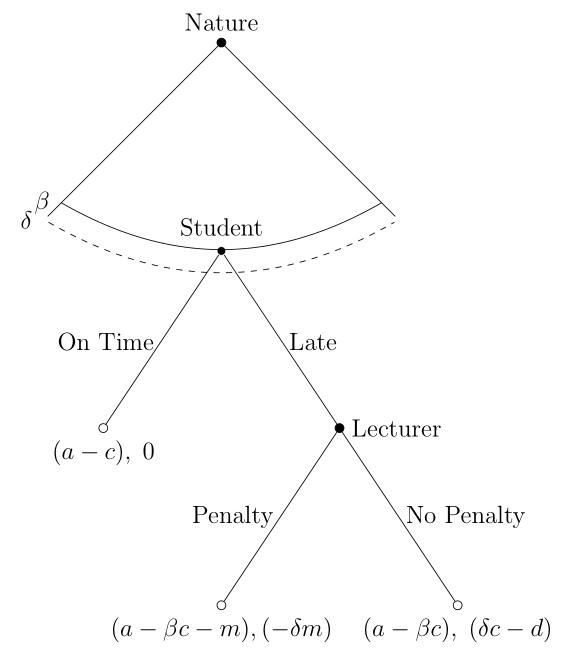
\includegraphics[scale=1.5]{"img/continuous.jpg"}
\captionof{figure}{This game is dynamic, where nature first chooses the student's and lecturer's types. The dashed line represents information only known by the lecturer and the solid line represents information only known by the student. Then the student moves, deciding to hand in on time or late after experiencing a crisis. If the student hands in late, the lecturer decides to impose a penalty or not. }
\label{Figure1}

\begin{table}[H]
\centering
\begin{tabular}{lll}
  \toprule
Parameter & Explanation & Restriction \\ 
  \midrule
$a$ & Potential assignment mark & $0\leq a \leq 1$ \\ 
  $c$ & Cost of crisis to assignment mark & $0 < c \leq 1$ \\ 
  $\beta$ & Student's type: level of resiliency & $\beta \sim Uniform(0,1)$  \\ 
  $m$ & Mark penalty & $0 < m \leq 1$ \\ 
  $\delta$ & Lecturer's type: level of empathy & $\delta \sim Uniform(0,1)$ \\ 
  $d$ & Detterent & $0<d \leq 1$ \\ 
   \bottomrule
\end{tabular}
\caption{Game Parameters \label{sum}} 
\end{table}

\hypertarget{results-and-discussion}{%
\section{\texorpdfstring{Results and Discussion
\label{result}}{Results and Discussion }}\label{results-and-discussion}}

In order to understand how the lecturer and student will make their
decisions given their beliefs, we need to solve for their best
responses. A best response for the student would be to hand in on time
if the expected payoff from handing in on time is higher than the
expected payoff of submitting late. Defining \(p\) as the probability
that the lecturer will give a penalty, a student should hand in on time
where: \begin{align*}
\beta>\frac{c-m p}{c}
\end{align*} The right hand side is a constant\footnote{Since \(c\) and
  \(m\) are known, and \(p\) is a belief the student holds.}. This
implies that there is some threshold value of \(\beta\), for which a
student should hand in on time. If the student believes that the
lecturer will give no penalty (i.e.~\(p=0\)), then she should only hand
in on time if \(\beta > \frac{c}{c} \Rightarrow \beta > 1\). Since
\(\beta\) lies between \(0\) and \(1\), the inequality will never hold
and she should always hand in late. From an intuitive stand point, this
makes sense: a student can never do worse by handing in late if there is
no penalty\footnote{Handing in late is weakly dominant.} but she will do
better to hand in late if she is resilient in any way (\(\beta < 1\))
and can partially recover from the crisis.

However, if the student believes that the lecturer will give a penalty
with some positive probability (\(p>0\)) then her decision to hand in on
time depends on her level of resiliency, the magnitude of the crisis and
the size of the penalty. As the cost of the crisis increases, the
threshold value increases (ceteris paribus), and the student becomes
more likely to hand in late (unless her she has a very low resiliency).
If the mark penalty is high, the threshold value is smaller, and the
student is more likely to hand in on time (unless is very resilient:
\(\beta\) is very low). We can analyse the lecturer's best response rule
similarly. The lecturer should impose a penalty where:\\
\begin{align*}
\delta<\frac{d}{c+m}
\end{align*} The threshold value for the lecturer is the ratio between
the deterrent factor and the sum of the crisis cost and the penalty
mark. If the deterrent factor is high relative to the cost of crisis and
the penalty mark, then the lecturer is more likely to give a penalty
(unless he is highly empathetic). If the cost of the crisis large and
the mark penalty is high relative to the deterrent factor, the lecturer
is more likely to waive the penalty (unless he has very low empathy
levels).

While the best response analysis is useful, if we want to understand the
outcome of the game and the player's strategies, we need to solve for
the Bayesian Nash Equilibrium (BNE). The full derivations of the
solution concepts are given in the appendix (\ref{B}).

After observing her private type, the student chooses the following
hand-in pattern:\\
\begin{align*}
s_{\beta}^{*}(\beta)=\left\{\begin{array}{lll}
\text{On time} & \text{if} & \beta>1-\frac{m d}{c^{2}+m c}  \\
\text{Late} & \text{if} & \beta \leq 1-\frac{m d}{c^{2}+m c} 
\end{array}\right.
\end{align*}

And the lecturer's BNE strategy is given by: \begin{align*}
s_{\delta}^{*}(\delta)=\left\{\begin{array}{lll}
\text{Penalty} & \text { if } & \delta<\frac{d}{c+m} \\
\text{No penalty} & \text { if } & \delta \geq \frac{d}{c+m}
\end{array}\right.
\end{align*}

When the lecturer and the student play their equilibrium strategies,
neither has an incentive to deviate and we get a Bayesian Nash
equilibrium. We would interpret the student's BNE strategy similarly to
her best response; however, her strategy profile only depends on her own
type and no longer on her beliefs about the lecturer's type. The
lecturer's best response function and equilibrium strategy profile are
the same because the lecturer observes whether the student hands in late
or not and therefore has no need to hold beliefs about when the student
will hand in.

\hypertarget{extension}{%
\section{\texorpdfstring{Extension
\label{extension}}{Extension }}\label{extension}}

We extend the game explained in section \ref{game} to account for grade
inflation. The lecturer has an incentive to inflate the marks of the
student since a higher grade is associated with the student giving a
positive evaluation of the lecturer which could lead to an increase in
salary and promotions. However, inflation the mark if ethically wrong
therefore the lecturer incurs cost \(\gamma\) if he decides to inflate.
If he decides to leave the mark unchanged, then he occurs a sympathy
cost \(\delta\). A student experiences a cost of \(\omega\) for asking
the lecturer and the lecturer experiences a cost of \(\phi\) of being
bothered by the lecturer. If the lecturer decides not to penalize the
student, then he will never choose to inflate a students mark. Knowing
this, a student that hands in late and receives no penalty will always
accept his mark. If a student hands-on time, a lecture will always leave
the mark unchanged at the request of the student, therefore the student
will always accept the mark. If the lecturer decides to penalize a late
student, the lecturer will choose to inflate a student's mark if the
moral cost is smaller than the empathy cost the lecturer experiences.
\[\gamma < \delta m \] If the moral cost that the lecturer experiences
is bigger than the empathy cost the lecturer experiences for giving a
penalty, then the lecturer is strict, otherwise the lecturer is lenient.
Therefore, a strict lecturer will not inflate a student mark but a
lenient lecture will.

A summary of the game's parameter's and restrictions are shown in table
\ref{table:ext} and the game is represented in Figure \ref{fig:extd}

\begin{table}
\caption{Extended Game Parameters}
\centering
\begin{tabular}{c c c} \hline
Parameter & Explanation & Restrictions \\
\hline 
\(\omega\) & Exogenous cost of asking for the lecturer for higher mark & 0 < \(\omega\) $\le$ 1 \\
\(\delta\) & Ethical cost of inflating students mark & 0 < \(\delta\) $\le$ 1 \\
\(\phi\) & Cost of annoyance lecture experience for student bothering him & 0 <\(\phi\) $\le$ 1 \\
x & Additional marks that student get when lecturer decides to inflates &  1 < x $\le$ 2 \\ [1ex]
\hline 
\end{tabular}
\label{table:ext}
\end{table}

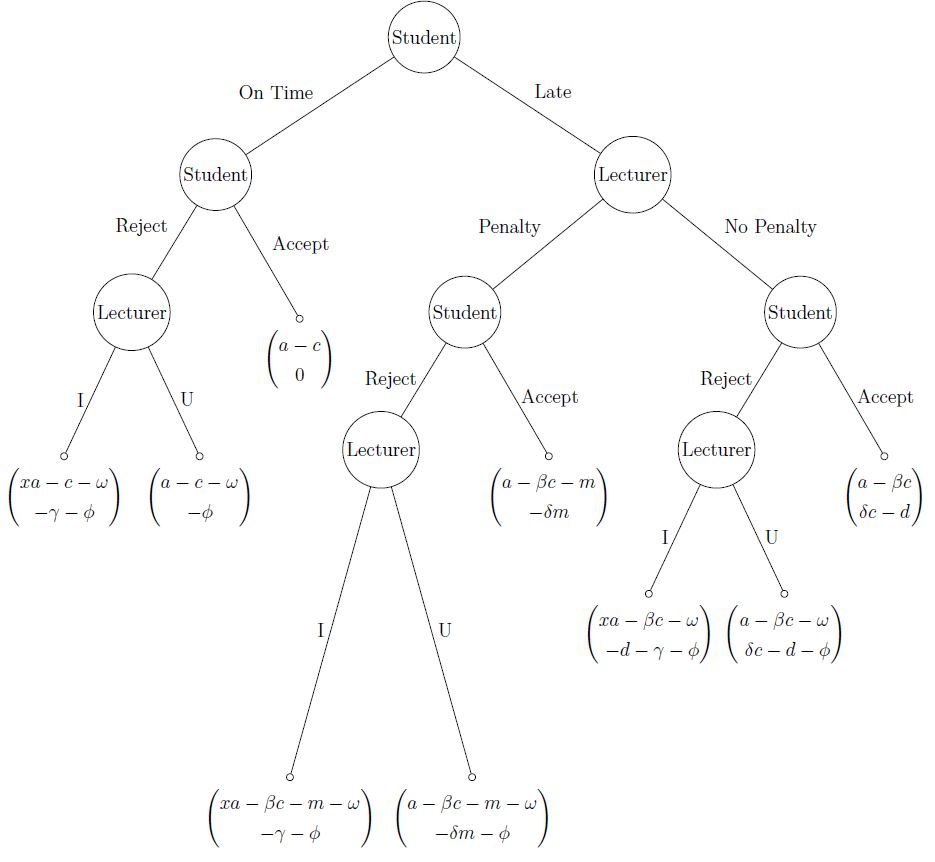
\includegraphics[scale=0.90]{"img/extend.jpg"}
\captionof{figure}{This is an extended version of the game presented in Figure 3.1. To account for grade inflation, the student gets to accept the grade the lecturer game him, or reject the grade and ask the lecturer for a better mark. The lectuerer can then decided to inflate (I) the students mark or leave the mark unchanged (U). }
\label{fig:extd}

\hypertarget{conclusion}{%
\section{\texorpdfstring{Conclusion
\label{con}}{Conclusion }}\label{conclusion}}

The results of the model are intuitive and provide a useful insight into
how student's think about handing in assignments, and how lecturers
respond to late submissions. One shortcoming of the model is its
assumption that \(c\) is common knowledge. Although some lecturers are
in touch with their students and would know whether they are
experiencing a crisis and how impactful the crisis would be, most
lecturers have too many students to know that information.

Extensions, generality Shortcomings \newpage

\hypertarget{references}{%
\section*{References}\label{references}}
\addcontentsline{toc}{section}{References}

\hypertarget{refs}{}
\begin{CSLReferences}{1}{0}
\leavevmode\hypertarget{ref-power}{}%
Conrad, C. 1983. Power and performance as correlates of supervisors'
choice of modes of managing conflict: A preliminary investigation.
\emph{Western Journal of Communication (includes Communication
Reports)}. 47(3):218--228.

\leavevmode\hypertarget{ref-comm}{}%
Conrad, C. 1991. Communication in conflict: Style-strategy
relationships. \emph{Communications Monographs}. 58(2):135--155.

\leavevmode\hypertarget{ref-harsanyi}{}%
Harsanyi, J.C. 1995. Games with incomplete information. \emph{The
American Economic Review}. 85(3):291--303. {[}Online{]}, Available:
\url{http://www.jstor.org/stable/2118175}.

\leavevmode\hypertarget{ref-trust}{}%
Liu, P. \& Shi, J. 2017. Trust in the subordinate and deference to
supervisor in china: A moderated mediation model of
supervisor-subordinate guanxi and political mentoring. \emph{Chinese
Management Studies}.

\leavevmode\hypertarget{ref-luce1956}{}%
Luce, R.D. \& Adams, E.W. 1956. The determination of subjective
characteristic functions in games with misperceived payoff functions.
\emph{Econometrica, Journal of the Econometric Society}. 158--171.

\leavevmode\hypertarget{ref-2004com}{}%
Myerson, R.B. 2004. Comments on ``games with incomplete information
played by `bayesian'players, i--III harsanyi's games with incoplete
information''. \emph{Management Science}. 50(12\_supplement):1818--1824.

\leavevmode\hypertarget{ref-book}{}%
Osborne, M.J. 2004. \emph{An introduction to game theory}. Vol. 3. (3).
Oxford university press New York.

\leavevmode\hypertarget{ref-2020games}{}%
Trabelsi, M. 2020. Games with incomplete information: A framework based
on possibility theory. PhD thesis. Universit{é} de Toulouse,
Universit{é} Toulouse III-Paul Sabatier.

\end{CSLReferences}

\newpage

\hypertarget{appendix-a}{%
\section*{\texorpdfstring{Appendix A
\label{A}}{Appendix A }}\label{appendix-a}}
\addcontentsline{toc}{section}{Appendix A \label{A}}

\begin{table}[H]
\centering
\begin{tabular}{rll}
  \toprule
 & Penalty & No Penalty \\ 
  \midrule
On Time & $a-c, \ 0$ & $a-c, \ 0$ \\ 
  Late & $a-\beta c - m, \ \delta m$ & $a-\beta c, \ \delta c -d$ \\ 
   \bottomrule
\end{tabular}
\caption{Strategic form of the game \label{tab1}} 
\end{table}

\hypertarget{appendix-b}{%
\section*{\texorpdfstring{Appendix B
\label{B}}{Appendix B }}\label{appendix-b}}
\addcontentsline{toc}{section}{Appendix B \label{B}}

\hypertarget{payoffs}{%
\subsection*{\texorpdfstring{Payoffs
\label{payoff}}{Payoffs }}\label{payoffs}}
\addcontentsline{toc}{subsection}{Payoffs \label{payoff}}

Student payoffs: \begin{align*}
E[\text{On Time}]&= a- c \\
E[\text{Late}]&=  p(a-\beta c-m) +(1-p)(a-\beta c) \\
&=-m p+a-\beta c
\end{align*} Student plays on time if: \begin{align*}
a-c>a-m p-\beta c \\
\beta c>c-m p \\
\beta>\frac{c-m p}{c}
\end{align*} Student plays late if: \begin{align*}
\beta<\frac{c-m p}{c}
\end{align*} Lecturer Payoffs: \begin{align*}
E[\text{Penalty}]&=q(-\delta m)+(1-q)(0) \\
&=q(-\delta m) \\
E[\text{No Penalty}] &=q(\delta c-d)+(1-a)(0) \\
&=q(\delta c-d)
\end{align*} Lecturer gives a penalty if: \begin{align*}
q(-\delta m)&>q(\delta c-d) \\
-\delta m&>\delta c-d \\
d&>\delta(c+m) \\
\delta&<\frac{d}{c+m} \\
\delta &<\bar{\delta}
\end{align*} Lecturer gives no penalty if: \begin{align*}
\delta &\geq \frac{d}{c+m} \\
\delta &\geq \bar{\delta} \\
\end{align*}

\hypertarget{best-responses}{%
\subsection*{\texorpdfstring{Best Responses
\label{br}}{Best Responses }}\label{best-responses}}
\addcontentsline{toc}{subsection}{Best Responses \label{br}}

Solving for the best responses: \begin{align*}
p=\text{Probability that the lecturer gives a penalty} = \bar{\delta}=\operatorname{Prob}(\delta<\bar{\delta})
\end{align*} Substitute into the student's best response function -
student hands in on time if: \begin{align*}{}
\beta>\frac{c-m(\bar{\delta})}{c}
\end{align*}{} Since \(0 \leq \beta \leq 1\), \(\beta\) cannot be
greater than 1. This implies \begin{align*}{}
\frac{c-m(\bar{\delta})}{c} \leq 1 \\
c-m \bar{\delta} \leq c \\
-m \bar{\delta} \leq 0 \\
0 \leq \bar{\delta}
\end{align*}{} Since \(0 \leq \bar{\delta} \leq 1\), this condition will
always hold.

\(\beta\) cannot be less than 0: \begin{align*}
\frac{c-m \bar{\delta}}{c}&<0 \\
c-m \bar{\delta}&<0 \\
-m \bar{\delta}&< -c \\
\bar{\delta}&>\frac{c}{m}
\end{align*} if \(\bar{\delta}>\frac{c}{m} \Rightarrow \beta=0\),
otherwise: \begin{align*}
\beta =\frac{c-m \bar{\delta}}{c}
\end{align*} Best response function for the student: \begin{align*}
B R_{\beta}(\bar{\delta})=\left\{\begin{array}{lll}
\frac{c-m\bar{\delta}}{c} & \text { if } & \bar{\delta}\leq \frac{c}{m} \\
0 & \text { if } & \bar{\delta}> \frac{c}{m}
\end{array}\right.
\end{align*} Best response function for the lecturer: \begin{align*}
B R_{\delta}(\delta)=\left\{\begin{array}{lll}
\text{Penalty} & \text { if } & \delta<\frac{d}{c+m} \\
\text{No penalty} & \text { if } & \delta \geq \frac{d}{c+m}
\end{array}\right.
\end{align*}

\hypertarget{bayesian-nash-equilibrium}{%
\subsection*{\texorpdfstring{Bayesian Nash Equilibrium
\label{bay}}{Bayesian Nash Equilibrium }}\label{bayesian-nash-equilibrium}}
\addcontentsline{toc}{subsection}{Bayesian Nash Equilibrium \label{bay}}

The Bayesian Nash equilibrium occurs at the point where the best
response functions intersect. For the BRFs to cross: \begin{align*}
\text{Substitute} \; \bar{\delta} &= \frac{d}{c+m} \; \text{into} \; \beta=\frac{c-m\bar{\delta}}{c} \\
\text{Then:} \; \beta&=\frac{c}{c}-\frac{m}{c}\left(\frac{d}{c+m}\right) \\
\beta&=1-\frac{m d}{c^{2}+m c} \\
\end{align*} BNE strategy for the student \begin{align*}
s_{\beta}^{*}(\beta)=\left\{\begin{array}{lll}
\text{On time} & \text{if} & \beta>1-\frac{m d}{c^{2}+m c} \\
\text{Late} & \text{if} & \beta \leq 1-\frac{m d}{c^{2}+m c}
\end{array}\right.
\end{align*} BNE strategy for the lecturer \begin{align*}
s_{\delta}^{*}(\delta)=\left\{\begin{array}{lll}
\text{Penalty} & \text { if } & \delta<\frac{d}{c+m} \\
\text{No penalty} & \text { if } & \delta \geq \frac{d}{c+m}
\end{array}\right.
\end{align*}

\bibliography{Tex/ref}





\end{document}
